\documentclass[../Bachelorarbeit.tex]{subfiles}
\begin{document}

\subsection{Kontextanalyse}
Ziel der Kontextanalyse ist die Abgrenzung des Kontexts \bzw das Finden von Systemgrenzen. Bei dem mehrachsigen Positioniersystem handelt es sich um ein sogenanntes eingebettetes System (\eng Embedded System). Diese kommunizieren meist stark mit ihrer Umwelt \bzw sind meist stark mit dieser verankert. % Quelle
So auch hat das Positioniersystem Schnittstellen, über die eine Kommunikation mit Nachbarsystemen stattfindet. In der Systemkonzeption muss folglich geklärt werden, wo genau die Systemgrenzen liegen. Weiterhin findet in der Kontextabgrenzung auch die Identifizierung von Nachbarsystemen statt.\\ % Quelle
Zuerst muss geklärt werden, ob die Systemumgebung dynamischer natur ist, das heißt, dass Nachbarsysteme wechseln \bzw das System nicht umgebungstreu ist. Handelt es sich im Gegensatz dazu um ein System mit stabiler Umgebung, ist die Darstellung von Nachbarsystemen simpel und kann nachfolgend im entsprechenden Diagramm dokumentiert werden. Da das mehrachsige Positioniersystem fest in den Laborraum integriert ist, und alle Nachbarsysteme bereits bekannt sind, wird in der Analyse von einer statischen Umgebung ausgegangen. Die sich anschließende Liste zeigt alle derzeitigen Nachbarsysteme, in die das mehrachsige Positioniersystem eingebettet ist.\\

\begin{itemize}
    \item Laborcomputer
    \item Ablageschale/Aufnahmeschale (Ablagepositionen)
    \item Externe Industriesteuerungen
    \item Augmented Reality Server
    \item Verwaltungsschalen (Digitaler Zwilling)
    \item mögliche spätere Erweiterung: Förderbänder
    \item mögliche spätere Erweiterung: Vorratslager (statt Aufnahmeschale)
    \item mögliche spätere Erweiterung: Lagermagazin(e) (statt Ablageschale)
\end{itemize}

Ist die Identifizierung der Nachbarsysteme abgeschlossen, kann mit der Kontextanalyse begonnen werden. Der Kontext unterteilt sich in den logischen Kontext und den physikalischen Kontext. Der \textbf{logische Kontext} betrachtet die Kommunikation mit den Nachbarsystemen, wohingegen der \textbf{physikalische Kontext} auf die Kommunikationshardware fokussiert ist.\\ % Quelle
Für die Dokumentation der logischen Kontextabgrenzung bietet sich sich das Anwendungsfalldiagramm der UML (Unified Modeling Language) an. Dabei handelt es sich um die allgemein gängige Form für diese Aufgabe. Das Anwendungsfalldiagramm bietet sich an dieser Stelle an für die Modellierung, da für die Darstellung noch keine detaillierten Entscheidungen über die Schnittstellen getroffen werden müssen. Es ist geeignet um das zu modellierende System und seine Nachbarsysteme in Beziehung darzustellen und deren Kommunikation grundlegend anzudeuten. \autoref{fig:my-img1} zeigt die logische Kontextabgrenzung des mehrachsigen Positioniersystems zu den bereits aufgezählten Nachbarsystemen mittels des Anwendungsfalldiagramms.\\ 

\begin{figure}[h]
    \centering
    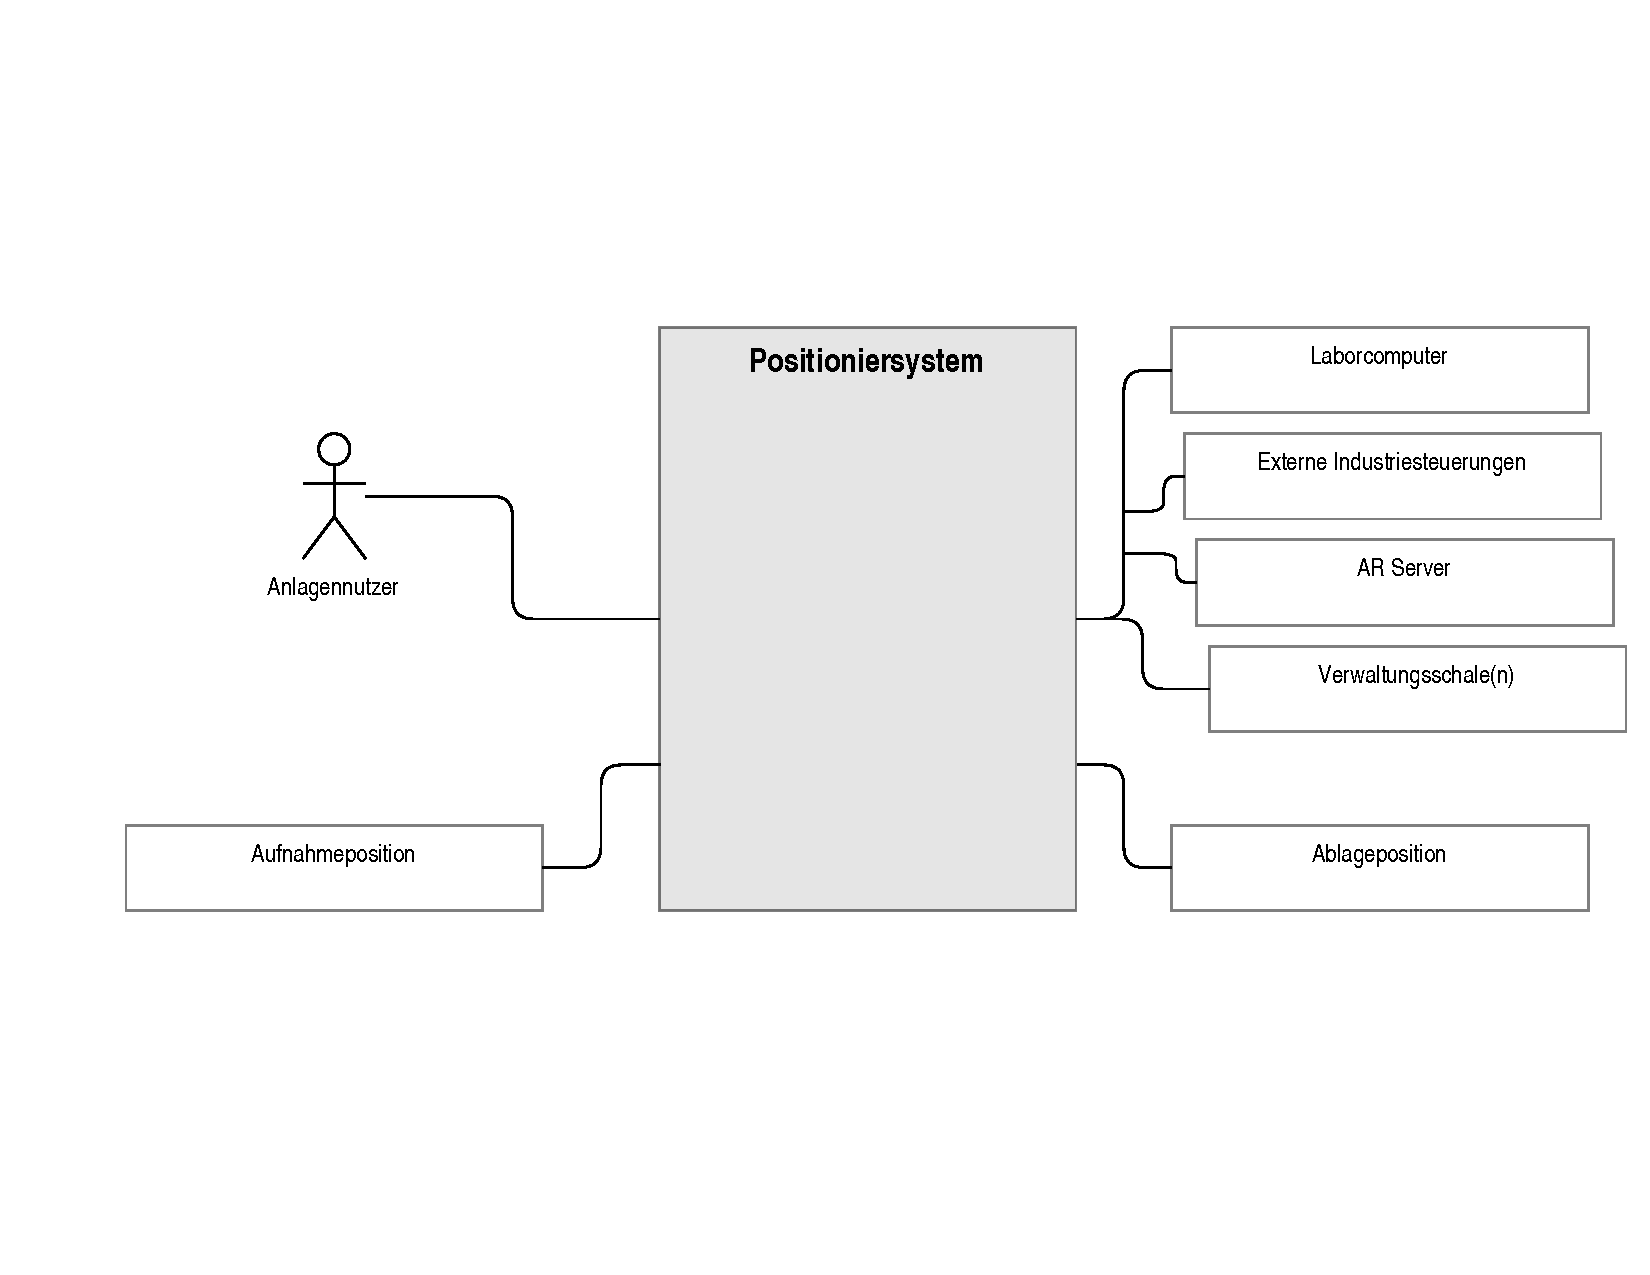
\includegraphics[width=\textwidth]{Images/kontextana.pdf}
    \caption[Logische Kontextabgrenzung]{Logische Kontextabgrenzung des mehrachsigen Positioniersystems}
    \label{fig:my-img1}
\end{figure}

\end{document}